\documentclass[tikz,border=6pt]{standalone}
% Shared visual language for the original benchmark atlas.
\usepackage[T1]{fontenc}
\usepackage{lmodern}
\usepackage{amsmath,amssymb}
\usetikzlibrary{arrows.meta,calc,positioning,shapes.geometric,patterns,decorations.pathmorphing,backgrounds,fit}
\definecolor{ink}{HTML}{173948}
\definecolor{flow}{HTML}{167D9A}
\definecolor{control}{HTML}{A65217}
\definecolor{measure}{HTML}{70518A}
\definecolor{pale}{HTML}{EAF2F5}
\definecolor{muted}{HTML}{526571}
\definecolor{utility}{HTML}{2E8665}
\tikzset{
  every node/.style={font=\sffamily\small,text=ink},
  equipment/.style={draw=ink,line width=1pt,fill=pale,rounded corners=2pt},
  process/.style={draw=flow,line width=1.2pt,-{Latex[length=2.5mm]}},
  signal/.style={draw=control,line width=.8pt,dashed,-{Latex[length=2mm]}},
  util/.style={draw=utility,line width=1pt,-{Latex[length=2.2mm]}},
  dimension/.style={draw=muted,line width=.6pt,{Latex[length=1.7mm]}-{Latex[length=1.7mm]}},
  labelbox/.style={fill=white,inner sep=2pt,font=\sffamily\footnotesize,align=center},
  annotation/.style={font=\sffamily\footnotesize,text=muted,align=left},
  panel/.style={draw=ink!20,fill=ink!2,rounded corners=3pt,inner sep=6pt},
  instrument/.style={circle,draw=measure,fill=white,line width=.8pt,minimum size=8mm,inner sep=1pt,font=\sffamily\scriptsize,align=center},
  port/.style={circle,fill=flow,inner sep=1.6pt},
  box/.style={equipment,minimum width=3cm,minimum height=1cm,align=center},
}
\newcommand{\atlasheader}[3]{%
  \node[anchor=north west,font=\sffamily\bfseries\LARGE] at (0,0) {#1};%
  \node[anchor=north west,font=\sffamily\small,text=muted] at (0,-.75) {Paper section #2: \textit{#3}};%
  \draw[ink!25,line width=.7pt] (0,-1.25)--(26,-1.25);%
}
\newcommand{\atlasfooter}[1]{%
  \draw[ink!25,line width=.5pt] (0,-15.8)--(26,-15.8);%
  \node[anchor=north west,annotation,text width=25.8cm] at (0,-16) {#1\\Original explanatory drawing. Source: Kroll \& Schulte (2014), DOI: 10.1016/j.asoc.2014.08.034. Model variants are identified in the accompanying case sheet.};%
}

\begin{document}
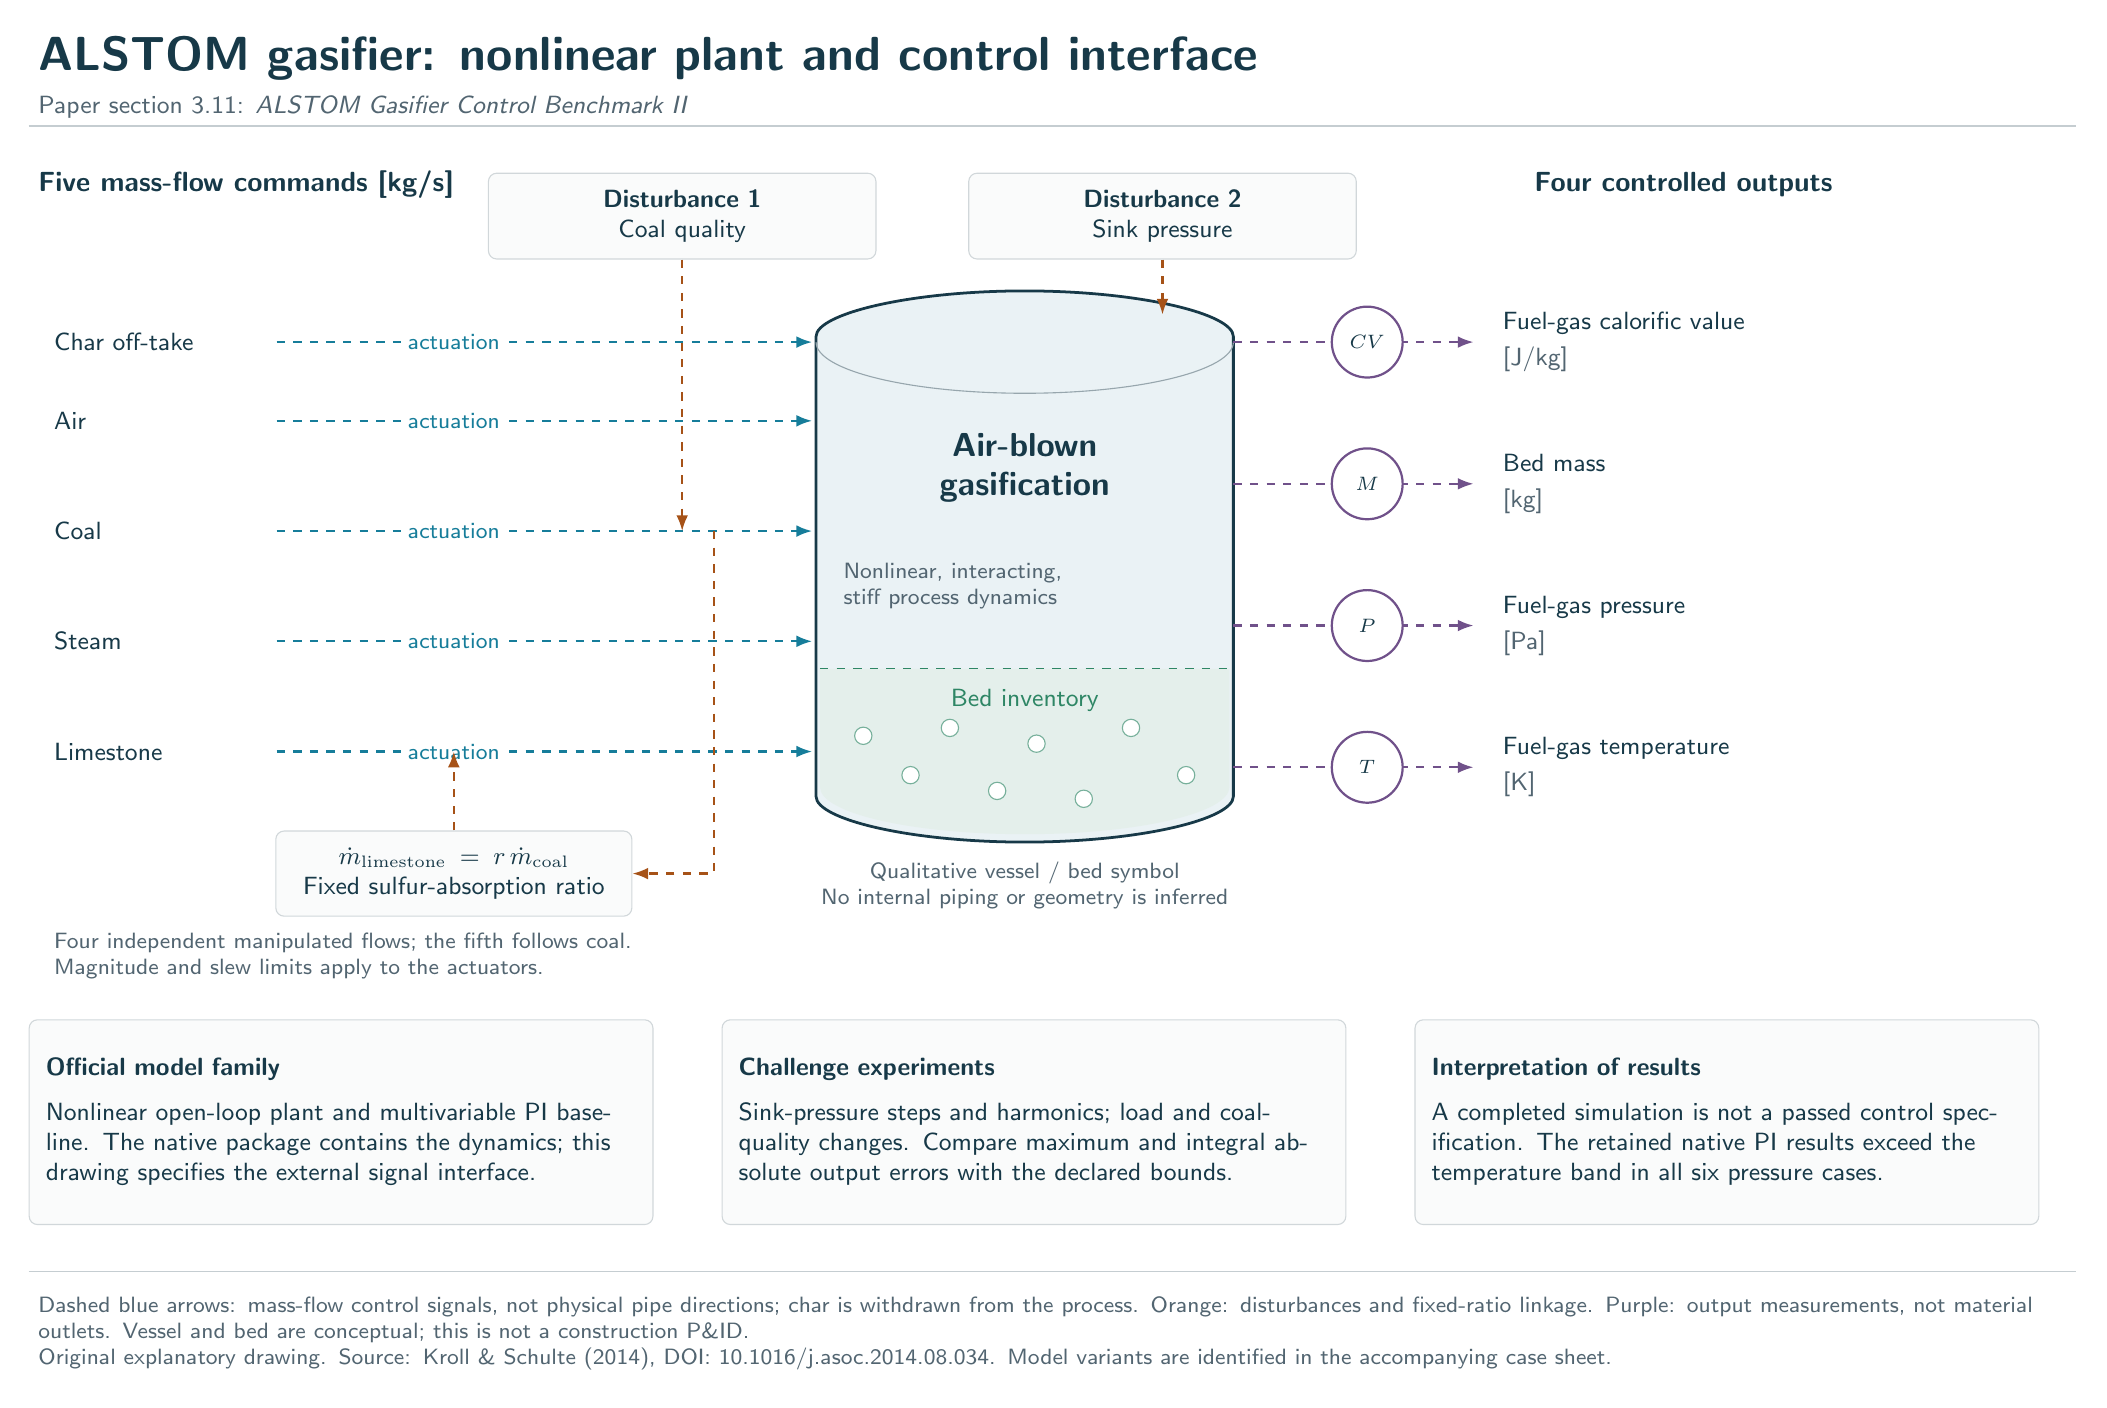
\begin{tikzpicture}[x=1cm,y=1cm]
\atlasheader{ALSTOM gasifier: nonlinear plant and control interface}{3.11}{ALSTOM Gasifier Control Benchmark II}
\node[anchor=west,font=\sffamily\bfseries] at (0,-2) {Five mass-flow commands [kg/s]};
\node[anchor=west,font=\sffamily\bfseries] at (19,-2) {Four controlled outputs};

% Vessel appearance is deliberately qualitative: only the interface is quantitative.
\path[equipment] (10,-4) arc[start angle=180,end angle=0,x radius=2.65cm,y radius=.65cm]
 --(15.3,-9.7) arc[start angle=0,end angle=-180,x radius=2.65cm,y radius=.65cm]--cycle;
\draw[ink!45] (10,-4) arc[start angle=180,end angle=360,x radius=2.65cm,y radius=.65cm];
\path[fill=utility!13] (10.05,-8.15) -- (15.25,-8.15) -- (15.25,-9.65)
 arc[start angle=0,end angle=-180,x radius=2.6cm,y radius=.6cm] --cycle;
\draw[utility,dashed] (10.05,-8.15)--(15.25,-8.15);
\foreach \x/\y in {10.6/-9.0,11.2/-9.5,11.7/-8.9,12.3/-9.7,12.8/-9.1,13.4/-9.8,14/-8.9,14.7/-9.5}
  \draw[utility!65,fill=white] (\x,\y) circle (.11);
\node[align=center,font=\sffamily\bfseries\large] at (12.65,-5.6) {Air-blown\\gasification};
\node[align=center,annotation,text width=4.6cm] at (12.65,-7.1) {Nonlinear, interacting,\\stiff process dynamics};
\node[align=center,font=\sffamily\small,text=utility] at (12.65,-8.55) {Bed inventory};
\node[annotation,align=center] at (12.65,-10.9) {Qualitative vessel / bed symbol\\No internal piping or geometry is inferred};

\foreach \yy/\lab in {-4.0/{Char off-take},-5.0/{Air},-6.4/{Coal},-7.8/{Steam},-9.2/{Limestone}}{
  \node[anchor=west] at (0.2,\yy) {\lab};
  \draw[signal,draw=flow] (3.15,\yy)--(9.95,\yy);
  \node[labelbox,font=\sffamily\footnotesize,text=flow] at (5.4,\yy) {actuation};
}
\node[panel,align=center,text width=4.1cm] (ratio) at (5.4,-10.75)
 {$\dot m_{\mathrm{limestone}}=r\,\dot m_{\mathrm{coal}}$\\Fixed sulfur-absorption ratio};
\draw[signal] (8.7,-6.4)--(8.7,-10.75)--(ratio.east);
\draw[signal] (ratio.north)--(5.4,-9.2);
\node[annotation,anchor=west,text width=7.6cm] at (0.2,-11.8) {Four independent manipulated flows; the fifth follows coal. Magnitude and slew limits apply to the actuators.};

\node[panel,align=center,text width=4.5cm] (coalquality) at (8.3,-2.4) {\textbf{Disturbance 1}\\Coal quality};
\node[panel,align=center,text width=4.5cm] (sinkpressure) at (14.4,-2.4) {\textbf{Disturbance 2}\\Sink pressure};
\draw[signal] (coalquality.south)--(8.3,-6.4);
\draw[signal] (sinkpressure.south)--(14.4,-3.65);
\foreach \yy/\sym/\lab/\un in {-4.0/{CV}/{Fuel-gas calorific value}/{J/kg},-5.8/{M}/{Bed mass}/{kg},-7.6/{P}/{Fuel-gas pressure}/{Pa},-9.4/{T}/{Fuel-gas temperature}/{K}}{
  \draw[signal,draw=measure] (15.3,\yy)--(18.35,\yy);
  \node[instrument,minimum size=9mm] at (17,\yy) {$\sym$};
  \node[anchor=west,align=left] at (18.6,\yy) {\lab\\[2pt]\textcolor{muted}{[\un]}};
}
\node[panel,anchor=north west,text width=7.5cm,minimum height=2.6cm,align=left] at (0,-12.6)
 {\textbf{Official model family}\\[5pt]
 Nonlinear open-loop plant and multivariable PI baseline. The native package contains the dynamics; this drawing specifies the external signal interface.};
\node[panel,anchor=north west,text width=7.5cm,minimum height=2.6cm,align=left] at (8.8,-12.6)
 {\textbf{Challenge experiments}\\[5pt]
 Sink-pressure steps and harmonics; load and coal-quality changes. Compare maximum and integral absolute output errors with the declared bounds.};
\node[panel,anchor=north west,text width=7.5cm,minimum height=2.6cm,align=left] at (17.6,-12.6)
 {\textbf{Interpretation of results}\\[5pt]
 A completed simulation is not a passed control specification. The retained native PI results exceed the temperature band in all six pressure cases.};
\atlasfooter{Dashed blue arrows: mass-flow control signals, not physical pipe directions; char is withdrawn from the process. Orange: disturbances and fixed-ratio linkage. Purple: output measurements, not material outlets. Vessel and bed are conceptual; this is not a construction P\&ID.}
\end{tikzpicture}
\end{document}
